\documentclass[xcolor=table]{beamer}
\usepackage{adjustbox}
\usepackage{comment}
\usetheme{Madrid}
\usepackage{wrapfig}
\usepackage{natbib}
\bibliographystyle{abbrvnat}
\setcitestyle{authoryear,open={},close={}}


\title{Graph Neural Network Applications}

% A subtitle is optional and this may be deleted
\subtitle{Master's Thesis}

\author{Pau~Rodriguez~Esmerats}


\institute[]
{
  Supervisor: Marta Arias Vicente\\
  \\
  Master in Innovation and Research in Informatics - Data Science\\
   Universitat Politecnica de Catalunya\\
  }

\date{October 2019}

\subject{}

\pgfdeclareimage[height=0.5cm]{./img/Logo_UPC}{./img/Logo_UPC}
\logo{\pgfuseimage{./img/Logo_UPC}}

\begin{comment}
\AtBeginSection[]
{
  \begin{frame}<beamer>{Outline}
    \tableofcontents[currentsection]
  \end{frame}
}
\end{comment}
\begin{comment}


\end{comment}

\begin{document}

\begin{frame}
  \titlepage
\end{frame}

\begin{frame}{Table of Contents}
  \tableofcontents
\end{frame}





%------------------------------------------------------------------------
\section{Introduction}
\begin{frame}{ }
\huge{1. Introduction}
\end{frame}


%------------------------------------------------------------------------
\begin{frame}{Introduction}{Graph Neural Networks definition}
    \begin{block}{What are Graph Neural Networks?}
    {
Graph Neural Networks allow to create an end to end machine
learning model that is simultaneously trained to learn a representation of graph structured data and to fit a predictive model on it.\\
They achieved state-of-the-art performance on semi-supervised learning and supervised graph classification.
}
    \end{block}


Successful applications of Graph Neural Networks:
\begin{itemize}
    \item Recommender systems
    \item Biochemistry
    \item Communication Networks
    \item Program verification
    \item Social Network analysis
\end{itemize}

\end{frame}


% %------------------------------------------------------------------------
% \begin{frame}{Introduction}
%     \begin{block}{What are Graph Neural Networks?}
%     {
%     % Main papers and their applications in topics/areas list 

%     % initial 2005, 2009    
%     % Bruan 
%     % GCN
%     % GraphSage
%     % Gin
%     % GGNN

%     }
%     \end{block}

% \end{frame}


%--------------------------------------------------------------------
\begin{frame}{Introduction}{Project definition}
    \begin{block}{Goal}
    {
    Explore Graph Neural Networks and apply them to different problems to create a novel solution. \\

     %The goal of this master’s thesis is to apply Graph Neural Network models to different problems to create a novel solution. The idea is to get to know how Graph Neural Networks are used in each situation. Two problems are explored: Girvan-Newmann algorithm approximation and compiled code function classification. They correspond to the two main tasks that Graph Neural Network perform with success, semi-supervised learning of nodes on a graph and supervised graph classification.        
    }
    \end{block}

    \begin{block}{Motivation}
    {
    Graph Neural Networks seem to be a promising way of solving graph-related problems, with applications in many domains. 

    % Graph Neural Networks seem to be a promising way of solving graph-related problems, with applications in many domains. 


    % data expressed as a graph is more exciting to me because it allows to express more complex real world phenomenon like 
    % complex network communications that have to be modelled by costly simulations or that have a huge combinatorial explosion when looking for solutions is overwhelming 
    % or knowledge that allow to represent knowledge and to reason about it

    % personal choice, kind of exciting to me, more than other machine learning tasks like for instance price forecasting, credit scoring

    % since there has been a lot of research in the last 2-3 years on that topic it seemed a good moment to look into thath




    }
    \end{block}

    Organization of the thesis:
        \begin{itemize}
            \item Overview of GNN (state of the art)
            \item Experiment 1 - Girvan-Newman algorithm approximation
            \item Experiment 2 - Compiled code function classification
        \end{itemize}

    % one does semi-supervised learning
    % the other does graph classification
    % and this is a way to get to know how main gnn models work, 

\end{frame}



% %------------------------------------------------------------------------REMOVE? -> TOC IS THE SAME
% \begin{frame}{Introduction}
%     \begin{block}{Organization}
%     {
% %      %The thesis is organized in the following way: the next section will explain the state-of-the-art in Graph Neural
% % Network models by presenting the may models, their internals and the problems they have solved. Then, in
% % section three, the methodology followed in the experiments is presented. After that, section four will go through
% % an overview of the implementation of the experiments, whereas in section five the results of the experiments are
% % summarized. Finally, in section six the conclusion of the thesis is presented.       
%     }
%     \end{block}
    
% \end{frame}



%------------------------------------------------------------------------
\section{State of the art}
\begin{frame}{ }
\huge{2. State of the art}
\end{frame}


%------------------------------------------------------------------------
\begin{frame}{State of the art}{Nomenclature}
% summarize Notation subsection from SOTA on report G,V,E,...

\textbf{Graph related concepts}
\vspace{15px}

\textbf{Graph:}  $G = (V,E,A)$ where $V$ is the set of nodes, $E$ is the set of edges and $A$ is the adjacency matrix. In a graph, let $ v_{i} \in V $ denote a node and $ e_{i,j} = (vi, vj) \in E $ denote an edge. 


\textbf{Adjacency matrix:} A is a $|V| \times |V|$ where $A_{i,j} = w_{i,j} > 0$ if $e_{i,j} \in E$ and $A_{i,j}=0$ if $e_{i,j} \notin E$.

\textbf{Node degree:} is the number of edges connected to it, $ degree(v_i) = \sum A_{i,:}$

And other related concepts: directed/undirected graph, isomorphism, etc.



\end{frame}
% \textbf{Directed graph:} all edges pointing from one node to another,  $ A_{i,j} \neq A_{j,i} $. 

% \textbf{Undirected graph:} all edges are bidirectional, $A_{i,j} = A_{j,i}$.

% \textbf{Isomorphism:} an isomorphism of graphs G and H is a bijection between the vertex sets of G and H $f:V(G) \to V(H)$ such that any two vertices u and v of G are adjacent in G if and only if f(u) and f(v) are adjacent in H (Wikipedia).

% \textbf{Node attributes:} X, where $X \in R^{|V| \times D}$ is a feature matrix with $X_i \in R^{D}$ representing the feature vector of node $v_i$. %In the case of $D = 1$, we replace $x \in R^N$ with X to denote the feature vector of the graph.
% We can also have edge attributes and graph-level atttributes.
%------------------------------------------------------------------------
\begin{frame}{State of the art}{Nomenclature}
%\begin{block}{ Machine learning concepts}{
\textbf{Machine learning concepts}
\vspace{15px}

\textbf{Node attributes:} X, where $X \in R^{|V| \times D}$ is a feature matrix with $X_i \in R^{D}$ representing the feature vector of node $v_i$. %In the case of $D = 1$, we replace $x \in R^N$ with X to denote the feature vector of the graph.
We can also have edge attributes and graph-level attributes.\\

\textbf{State:} we will define the state based on the values of the attributes on each node, edge or graph.

\textbf{Semi-supervised learning:} a supervised learning task with very few known target values. 

%}\end{block}


\end{frame}



% %------------------------------------------------------------------------
% \begin{frame}{State of the art}{Euclidean space}
% % Euclidean space definition
% % why Graph are considered non Euclidean

% %avoid??

% \end{frame}


%------------------------------------------------------------------------
\begin{frame}{State of the art}{Graph Neural Networks overview}

%\vspace{-10px}
\textbf{Common Graph Neural Network architecture}
% Usual architecture: embedding + downstream ML algorithm
\begin{figure}
    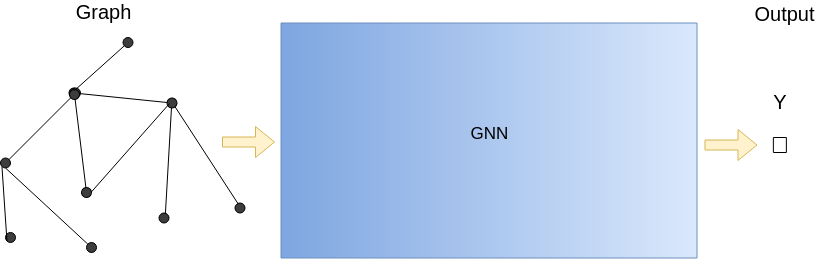
\includegraphics[scale=0.37]{./img/GNN_explanation_01b.png}
\end{figure}

\vspace{8px}
Tasks:
\begin{itemize}
    \item supervised graph classification or regression
\end{itemize}

\end{frame}



%------------------------------------------------------------------------
\begin{frame}{State of the art}{Graph Neural Networks overview}

\textbf{Common Graph Neural Network architecture}
% Usual architecture: embedding + downstream ML algorithm
\begin{figure}
    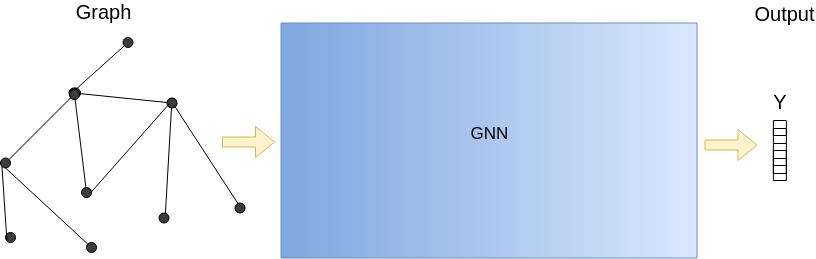
\includegraphics[scale=0.37]{./img/GNN_explanation_01.png}
\end{figure}


% tasks: node classif/regr, (sub)graph classif/regre 
%       -> repr. learning
% setupt: semi-supervised node repr. learning, and supervised graph repr. learning

\vspace{-10px}
Tasks:
\begin{itemize}
    \item supervised node classification/regression
    \item semi-supervised node classification/regression
\end{itemize}

% \begin{figure}[H]
% \minipage{0.5\textwidth}
% \begin{itemize}
%     \item supervised node classification/regression
%     \item supervised graph classification/regression
% \end{itemize}
% \endminipage
% \hfill
% \minipage{0.5\textwidth}%
% \begin{itemize}
%     \item semi-supervised node classification/regression
%     \item visualization 
% \end{itemize}
% \endminipage
% \end{figure}


\end{frame}





%------------------------------------------------------------------------
\begin{frame}{State of the art}{Graph Neural Networks overview}

\textbf{Common Graph Neural Network architecture}
% Usual architecture: embedding + downstream ML algorithm
\begin{figure}
    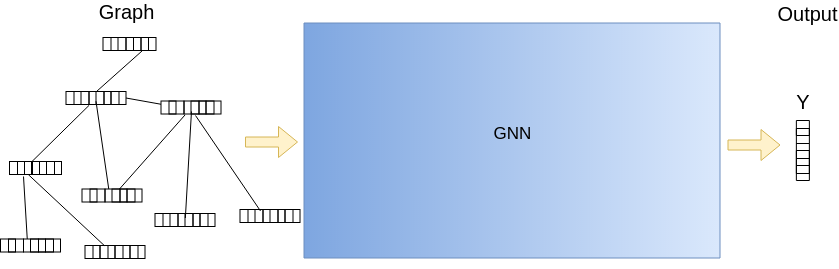
\includegraphics[scale=0.37]{./img/GNN_explanation_02.png}
\end{figure}
\vspace{-10px}
Tasks:
\begin{itemize}
    \item supervised node classification/regression
    \item semi-supervised node classification/regression
\end{itemize}

\end{frame}



%------------------------------------------------------------------------
\begin{frame}{State of the art}{Graph Neural Networks overview}

\textbf{Common Graph Neural Network architecture}
% Usual architecture: embedding + downstream ML algorithm
\begin{figure}
    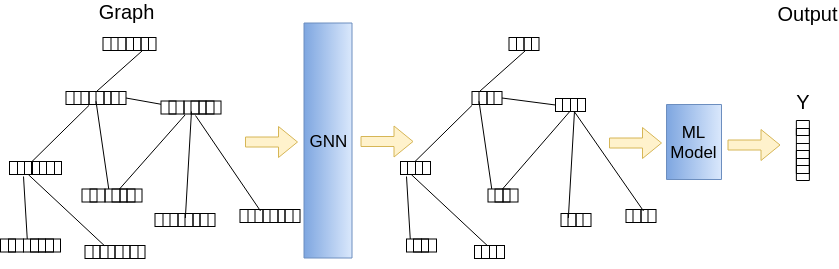
\includegraphics[scale=0.37]{./img/GNN_explanation_03.png}
\end{figure}
\vspace{-10px}
Tasks:
\begin{itemize}
    \item supervised node classification/regression
    \item semi-supervised node classification/regression
\end{itemize}

\end{frame}


%------------------------------------------------------------------------
\begin{frame}{State of the art}{Graph Neural Networks overview}

\textbf{Common Graph Neural Network architecture}
% Usual architecture: embedding + downstream ML algorithm
\begin{figure}
    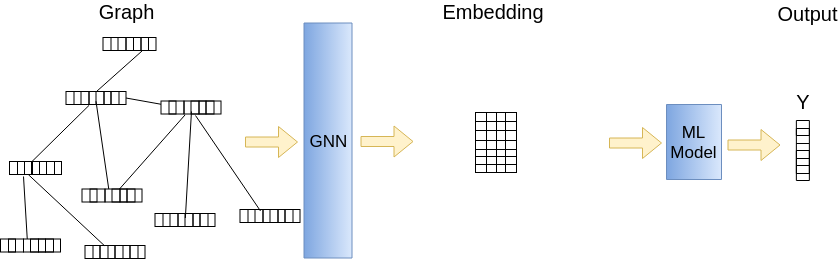
\includegraphics[scale=0.37]{./img/GNN_explanation_04.png}
\end{figure}
\vspace{-10px}
Tasks:
\begin{itemize}
    \item supervised node classification/regression
    \item semi-supervised node classification/regression
\end{itemize}

\end{frame}



%------------------------------------------------------------------------
\begin{frame}{State of the art}{Graph Neural Networks overview}

\textbf{Common Graph Neural Network architecture}
% Usual architecture: embedding + downstream ML algorithm
\begin{figure}
    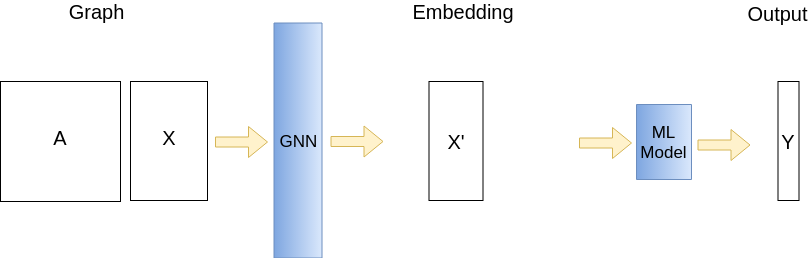
\includegraphics[scale=0.35]{./img/GNN_explanation_05.png}
\end{figure}
\vspace{-10px}
Tasks:
\begin{itemize}
    \item supervised node classification/regression
    \item semi-supervised node classification/regression
\end{itemize}

\end{frame}







%------------------------------------------------------------------------
\begin{frame}{State of the art}{Graph Neural Networks internals}

\textbf{Basic Graph Neural Network Layer Definition}
\begin{figure}
    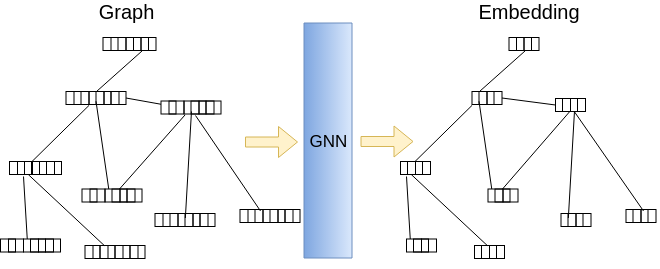
\includegraphics[scale=0.35]{./img/GNN_internals_01.png}
\end{figure}
\vspace{20px}
Let's look into the internals of Graph Neural Network layers alone.
\textbf{Observation:} a GNN layer corresponds to one iteration of the whole representation generation process. 
\end{frame}




%------------------------------------------------------------------------
\begin{frame}{State of the art}{Graph Neural Networks internals}

\textbf{Basic Graph Neural Network Layer Definition}

\begin{columns}
\column{0.5\textwidth}
\begin{figure}
    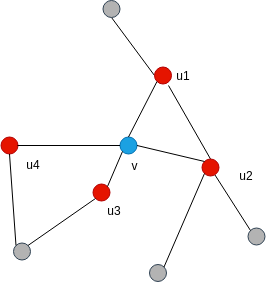
\includegraphics[scale=0.35]{./img/GNN_internals_02.png}
\end{figure}


\column{0.5\textwidth}
$ v $ is the current node that we are updating\\
$ u \in N(v)$ is the set of neighbor nodes of $v$\\


\end{columns}

\vspace{20px}
Generating the representation(embedding) of the nodes/graph:

\begin{enumerate}
    \item $ a_v^{(k)} = AGGREGATE^{(k)}(\{ h_u^{(k-1)} : u \in N(v) \}) ,$
    \item $ h_v^{(k)} = COMBINE^{(k)}(h_v^{(k-1)}, a_v^{(k)}),$
    \item $ h_G = READOUT(\{h_v^{(K)} | v \in G\})$  for graph level representation
\end{enumerate}
\vspace{20px}
Originally, those steps are iterated until convergence.
\end{frame}


%------------------------------------------------------------------------
\begin{frame}{State of the art}{Graph Neural Networks internals}

\textbf{Basic Graph Neural Network Layer Definition}

\begin{columns}
\column{0.5\textwidth}
\begin{figure}
    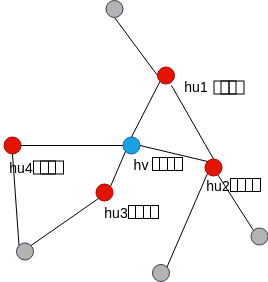
\includegraphics[scale=0.35]{./img/GNN_internals_03.png}
\end{figure}


\column{0.5\textwidth}
$ v $ is the current node that we are updating\\
$ u \in N(v)$ is the set of neighbor nodes of $v$\\
$h_u(k)$ is the state of node u at step(layer) $k$\\


\end{columns}

\vspace{20px}
Generating the representation(embedding) of the nodes/graph:

\begin{enumerate}
    \item $ a_v^{(k)} = AGGREGATE^{(k)}(\{ h_u^{(k-1)} : u \in N(v) \}) ,$
    \item $ h_v^{(k)} = COMBINE^{(k)}(h_v^{(k-1)}, a_v^{(k)}),$
    \item $ h_G = READOUT(\{h_v^{(K)} | v \in G\})$  for graph level representation
\end{enumerate}
\vspace{20px}
Originally, those steps are iterated until convergence.
\end{frame}







%------------------------------------------------------------------------
\begin{frame}{State of the art}{Graph Neural Network types}

These are the basic types of Graph Neural Networks:


\begin{itemize}
    \item \textbf{Original model}: iterates until convergence and no parameter sharing ( \citet{gori} , \citet{scarcelli}  )
    \item \textbf{Convolutional approach}: parameter sharing and limiting the iteration steps
        \begin{itemize}
            \item \textbf{Spectral-based methods}: matrix factorization approach (\citet{bruna}  )
            \item \textbf{Spatial-based methods}: neighborhood aggregation approach (\citet{gcn} , \citet{graphsage} )
        \end{itemize}
\end{itemize}
\end{frame}
% p6 sota GCN definition

% clarification: Kipf GCN versus broad type of convolutional networks
% convolution: sharing parameters



% %------------------------------------------------------------------------
% \begin{frame}{State of the art}{Spectral methods}

% % spectral methods characteristics pros and cons
% Spectral-based graph convolution methods are created like signal processing filters.
% \begin{itemize}
%     \item Based on the eigen-decomposition of the Laplacian matrix.
%     \item Drawback: any modification of the graph changes the eigenvector basis, can only be applied to graphs with same structure.
%     \item Drawback: all the graph must be in memory (scalability problem).
%     \item Drawback: limited to work on undirected graphs
% \end{itemize}
% %graph convolution operation is interpreted as removing noise from graph signals.
% %They rely on the eigen-decomposition of the Laplacian matrix. This has the drawback that any perturbation of
% %a graph results in a change of eigen basis, and the learned filters are domain dependent so they can’t be applied
% %to a graph with a different structure.

% \end{frame}


% %------------------------------------------------------------------------
% \begin{frame}{State of the art}{Spatial methods}
% % spatial methods pros and cons

% Spatial-based graph convolutions are based on the aggregation of nodes's spatial relations(neighbors).
% \begin{itemize}
%     \item Advantage: some spatial-based methods can generalize to unseen graph structures.
%     \item Advantage: aggregation of neighbors allows for processing large graphs by batches of nodes
%     \item Advantage: can be used on directed and undirected graphs.
% \end{itemize}

% \end{frame}





%------------------------------------------------------------------------
\begin{frame}{State of the art}{Graph Neural Network Implementations}

\textbf{The most common Graph Neural Network implementations are:}
\begin{itemize}
    \item Graph Convolutional Network (GCN)
    \item GraphSage
    \item Graph Isomorphism Network (GIN)
    \item Gated Graph Neural Network (GGNN)
    \item Message Passing Neural Network (MPNN)
\end{itemize}


\end{frame}




%------------------------------------------------------------------------
\begin{frame}{State of the art}{Graph Neural Networks Alternatives}
\textbf{There are mainly 3 alternatives:}
% alternatives quick mention: hand-engineerred features, kernel funcs, markov-random walk embeddings
\begin{itemize}
    \item Summary graph statistics (topological features)
    \item Kernel functions
    \item Network embeddings: matrix factorization and random walks
\end{itemize}
\vspace{15px}
They are precomputed or preconfigured. They don't adapt to the data!

\end{frame}






% %------------------------------------------------------------------------
% \begin{frame}{State of the art}{Spatial methods - GIN}

% %highlights
% \textbf{Graph Isomorphism Network:} implements the Weisfeiler-Lehman algorithm on graphs, used to detect isomorphisms (\citet{powerful}).
 
% %formula
% The node states are computed by:
% $$H^{(k)} = f(H^{(k-1)},A) =  \sigma(AH^{(k-1)}W^{(k-1)}),$$

% where $W^{(k)}$ is a weight matrix for the lth neural network layer and  $\sigma()$ is a non-linear activation function.


% \begin{figure}[H]
%     \centering
%         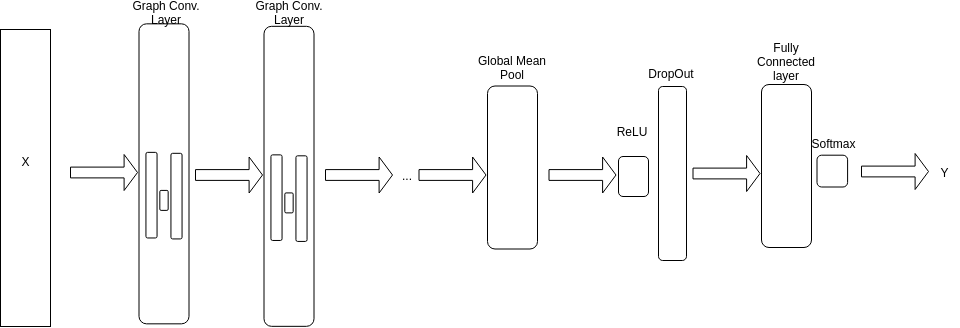
\includegraphics[width=0.75\linewidth]{img/GN_exp2_GIN.png}
%     \caption{Architecture of the Graph Isomorphism Network (GIN) model}\label{fig:gin_diagram}
% \end{figure}


% % what each layer represents (iterative steps)



% \end{frame}


% %------------------------------------------------------------------------
% \begin{frame}{State of the art}{Spatial methods - GCN}

% %highlights 
% \textbf{Graph Convolutional Network:} uses filter parameters $W^{(k)}$ that are shared over all locations in the graph (\citet{gcn}).

% %formula
% $$ h^{(k)}_{v_i} = \sigma(\sum_j \frac{1}{c_{ij}}h^{(k-1)}_{v_j}W^{(k-1)})$$

% where j indexes the neighboring nodes of $v_i$, and $c_{ij}$ is a normalization constant for the edge $(v_i,v_j)$.


% % generality of the GIN vs the constrained GCN
% % conditions that make GCN work
% % notes on where to look for specific explanations

% \end{frame}






% %------------------------------------------------------------------------
% \begin{frame}{State of the art}{Spatial methods - MPNN}

% %highlights 
% \textbf{Message Passing Neural Networks (MPNN):} The MPNN model generalizes several existing graph convolution networks into a unified framework named Message Passing Neural Network (\citet{mpnn}.

% %formula
% $$ h_v^t = U_t(h_v^{(t-1)}, \sum_{w \in N(v)} M_t(h_v^{t-1}, h_w^{t-1}, e_{vw}))$$


% \begin{figure}
%     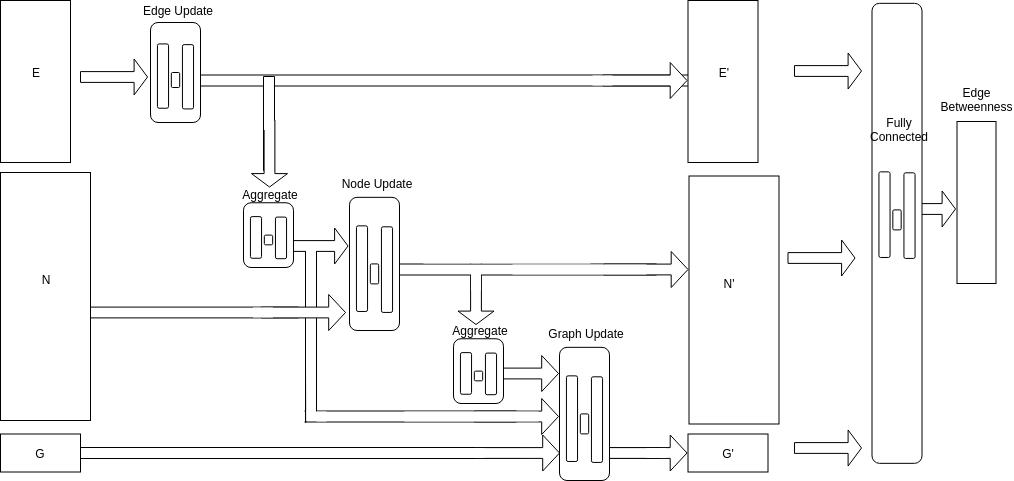
\includegraphics[width=0.6\linewidth]{img/GN_exp1_metalayer2.png}
% \caption{MPNN implementation as the MetaLayer model in Pytorch Geometric}
% \end{figure}

% % the implementation used effectively recreates the spatial based convolutional model on edge attributes and node attributes. But any other approach could be taken

% \end{frame}


% %------------------------------------------------------------------------
% \begin{frame}{State of the art}{Spatial methods - GraphSage}

% %highlights 
% %formula

% \end{frame}




% %------------------------------------------------------------------------
% \begin{frame}{State of the art}{Spatial methods - GGNN}

% %highlights
% \textbf{Gated Graph Neural Networks (GGNN):} emplois the gated recurrent units (GRU) \citet{GRU} as the recurrent function, reducing the recurrence to a fixed number of steps. The spatial graph convolution of GGNNs is defined as:

% %formula
% $$ h_v^t = GRU(h_v^{(t-1)}, \sum_{u \in N(v)} Wh_u^t) $$ 

% Uses back-propagation through time (BPTT) to learn the parameters.\\
% Costly and especially problematic for large graphs. 


% \end{frame}






% %------------------------------------------------------------------------
% \begin{frame}{State of the art}{Other GNNs}

% % G attention networks
% % G AUto-encoders
% % G Generative Networks
% % G spatial-temporal networks
% \end{frame}


% %------------------------------------------------------------------------
% \begin{frame}{State of the art}{Successful applications of GNN}

% %CV
% %Recsys
% % BIochemistry
% % Communication Networks modelling
% % Program verification
% \end{frame}




%------------------------------------------------------------------------
\section{Experiments}
\begin{frame}{ }
\huge{3. Experiments}
\end{frame}




% %------------------------------------------------------------------------REMOVE(go directly to first experiment)
% \begin{frame}{Experiments}


% \begin{itemize}
%     \item Experiment 1 - Girvan-Newman algorithm approximation
%     \item Experiment 2 - Compiled code function classification
% \end{itemize}

%     % \begin{block}{General goal}{
%     % % Apply GNN to 2 experiments: one covering semi-supervised node regression(classification)
%     % % the other covering supervised graph classification in the domain :

%     % }\end{block}
%     % \begin{block}{General motivation}{
%     %     % Make use of those great GNN algorithms in novel ways by applying them to new areas

%     % }\end{block}
%     % \begin{block}{Methodology}{
%     %     % adaptation of CRIPS-DM without business understanding and deployment
%     %     % for model selection & evaluation: hyper-parameter search with cross-validation for each type of model
%     %     % types of models: from simple baselines to more complex ones
%     % }\end{block}

% \end{frame}




%------------------------------------------------------------------------
\begin{frame}{Experiment 1 - Girvan-Newman algorithm approximation }{}

% Girvan-newman algorithm
\begin{block}{Girvan-Newman algorithm approximation}{
       Using Graph Neural Networks to approximate the Girvan-Newman algorithm for community detection in graphs.
    }\end{block}


\end{frame}




%------------------------------------------------------------------------
\begin{frame}{Experiment 1 - Girvan-Newman algorithm approximation }{ Context}

% Girvan-newman algorithm
\begin{block}{Girvan-Newman algorithm}{
        Clustering based approach algorithm for community detection that iteratively isolates groups of nodes of a graph by removing the edge with highest edge betweenness.
    }\end{block}


\begin{itemize}
    \item Edge betweenness: number of shortest paths between pairs of nodes that run along an edge
    \item Girvan-Newman time complexity: $O(m^{2}n)$ with $m$ edges and $n$ vertices
    %computing all the shortest paths that run along each edge is very costly, and must be recomputed at each iteration
\end{itemize}


\end{frame}



%------------------------------------------------------------------------
\begin{frame}{Experiment 1 - Girvan-Newman algorithm approximation }{ Goals and motivation}

\begin{itemize}
    % Goal: find a novel way to approximate the GN algorithm
    \item \textbf{Goal:} approximate the edge betweenness computation used in the Girvan-Newman algorithm by using Graph Neural Networks. 
    % show that it is possible
    % see how good the approximation is
    % see if the time cost is reduced
    \item \textbf{Motivation:} community detection is a popular task in social network analysis. Reducing the time cost of this algorithm would be very useful.
    % motivation: community detection popular task
\end{itemize}


\end{frame}



%------------------------------------------------------------------------
\begin{frame}{Experiment 1 - Girvan-Newman algorithm approximation }{ Description}


The implementation of the Girvan-Newman approximation would be:
\begin{itemize}
    \item Compute the edge betweenness of some edges of the graph
    \item Approximate the edge betweenness of the rest of edges of the graph (model prediction).
    \item Selection of the most central edge, and iterate.
\end{itemize}

\end{frame}




%------------------------------------------------------------------------
\begin{frame}{Experiment 1 - Girvan-Newman algorithm approximation }{ Description}


A Graph Neural Network has been trained to approximate the edge betweenness computation with a \textbf{semi-supervised node classification} task.\\

Discrete ranges of values of the edge betweenness are generated by percentiles.\\

% better performance if doing classification

\end{frame}






%------------------------------------------------------------------------
\begin{frame}{Experiment 1 - Girvan-Newman algorithm approximation }{ Results}


\begin{table}[H]
\adjustbox{max height=\dimexpr\textheight-5.9cm\relax,
           max width=0.99\textwidth, center}{

\centering
\begin{tabular}{|llllccc|}
\hline
 Model &                                                                          Paramteres  &  Runs\/Epochs  &  Splits &    Loss &        Accuracy &        F1-macro  \\
\hline
 META1 &      d19d16h10e19n16n15 & 100-20 & 100-2000-10556- &  2.3561 &   0.280 ± 0.061 &   0.251 ± 0.060  \\
 META1 &     d19d16h10e19n16n15 & 100-250 & 100-2000-10556- &  3.8995 &   0.139 ± 0.018 &   0.128 ± 0.020  \\
 META1 &         d19d16h10e19n16n15 & 100-20 & 20-500-1500- &  3.0269 &   0.142 ± 0.027 &   0.127 ± 0.029  \\
 META1 &        d19d16h10e19n16n15 & 100-250 & 20-500-1500- &  4.9482 &   0.093 ± 0.013 &   0.087 ± 0.017  \\
 META1 &      d19d16h10e19n16n15 & 100-20 & 200-3000-10556- &  2.0677 &  \textbf{ 0.342 ± 0.078} &   \textbf{0.312 ± 0.076 } \\
 META1 &     d19d16h10e19n16n15 & 100-250 & 200-3000-10556- &  3.3414 &   0.219 ± 0.027 &   0.208 ± 0.028  \\
 META1 &    d19d16h10e19n16n15 & 100-600 & 200-3000-10556- &  3.7691 &   0.142 ± 0.037 &   0.124 ± 0.039  \\
 META1 &    d19d16h10e19n16n15 & 100-2 & 20-500-10556- &  3.0165 &   0.112 ± 0.047 &   0.088 ± 0.052 \\
\hline
\end{tabular}
}
\label{Experiment1-v2}\caption{Edge betweenness approximation with a graph neural network experiment using 28 discrete ranges}
\end{table} 


\end{frame}





%------------------------------------------------------------------------
\begin{frame}{Experiment 1 - Girvan-Newman algorithm approximation }{ Results}


\begin{figure}[H]
\minipage{0.32\textwidth}%
  \centering
    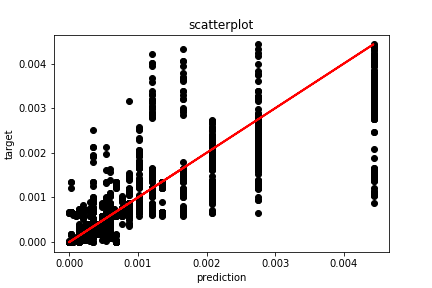
\includegraphics[width=0.9\linewidth]{img/GN_exp1/28bins/scatter_plot_20epochs.png}
\endminipage
\minipage{0.32\textwidth}%
  \centering
    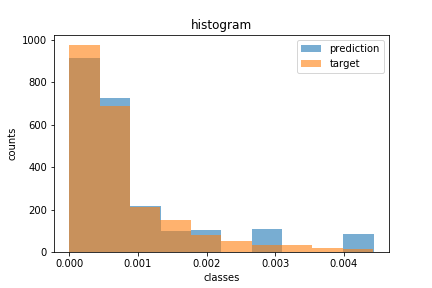
\includegraphics[width=0.9\linewidth]{img/GN_exp1/28bins/histogram_20epochs.png}
\endminipage
\minipage{0.32\textwidth}%
  \centering
    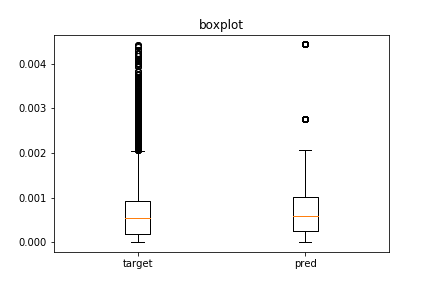
\includegraphics[width=0.9\linewidth]{img/GN_exp1/28bins/boxplot_20epochs.png}
\endminipage
\caption{Predictions compared to target values in an approximation of the edge betweenness using 28 discrete ranges and 20 epochs of training (best accuracy model) }\label{fig:edgeb_exp1_10bins}
\end{figure}

\end{frame}



%------------------------------------------------------------------------
\begin{frame}{Experiment 1 - Girvan-Newman algorithm approximation }{ Results}


\begin{figure}[H]
\minipage{0.32\textwidth}%
  \centering
    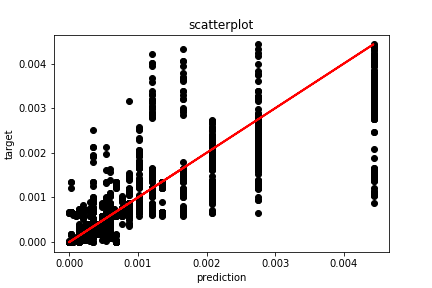
\includegraphics[width=0.9\linewidth]{img/GN_exp1/28bins/scatter_plot_20epochs.png}
\endminipage
\minipage{0.32\textwidth}%
  \centering
    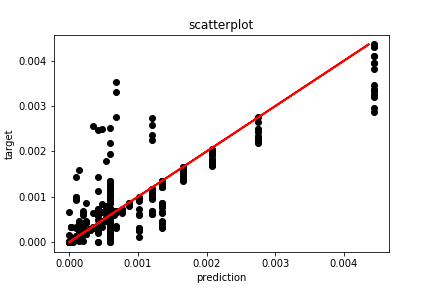
\includegraphics[width=0.9\linewidth]{img/GN_exp1/28bins/scatter_plot_250epochs.png}
\endminipage
\minipage{0.32\textwidth}%
  \centering
    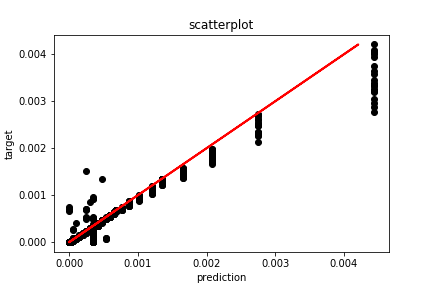
\includegraphics[width=0.9\linewidth]{img/GN_exp1/28bins/scatter_plot_600epochs.png}
\endminipage
\caption{Predictions compared to target values in an approximation of the edge betweenness using 28 ranges with 20, 250 and 650 epochs of training}\label{fig:edgeb_exp1_20bins}
\end{figure}

\end{frame}




%------------------------------------------------------------------------
\begin{frame}{Experiment 1 - Girvan-Newman algorithm approximation }{ Conclusion}


\textbf{What are the key take aways?}
% how good/bad is it?
\begin{itemize}
    \item The best trained model obtains a 34.3\% accuracy in a 28 discrete ranges setup.
    \item Limitation: the maximum edge betweenness is assigned to a group of edges and there is a limit on the number of discrete ranges that can be used.
    \item Model performance is highly dependent on the dataset split.
\end{itemize}
% how it could be improved even more?

\end{frame}

%------------------------------------------------------------------------
\begin{frame}{Experiment 1 - Girvan-Newman algorithm approximation }{ Next steps}



\textbf{How can the results be improved?}
% ways to apply this to Girvan-Newman approximation
\begin{itemize}
    \item Perform a longer hyper-parameter search.
    %\item Study if there is a better data partitioning approach 
    \item Test the model on different heterogeneous graphs to see how stable the model is.
    \item Create a smaller range for high edge betweenness values (and compensate for class imbalance).
    \item Use a different performance metric that benefits the detection of high edge betweenness values.
    \item Test an inductive setting.
\end{itemize}
\end{frame}






%------------------------------------------------------------------------
\begin{frame}{Experiment 2 - Compiled code function classification}{}


\begin{block}
    {
    Compiled code function classification
     }
    {
        Assembler code snippets renaming using Graph Neural Networks for graph classification

    }
\end{block}


\end{frame}





%------------------------------------------------------------------------
\begin{frame}{Experiment 2 - Compiled code function classification}{Context}

%Malicious software analysis overview


\begin{figure}
    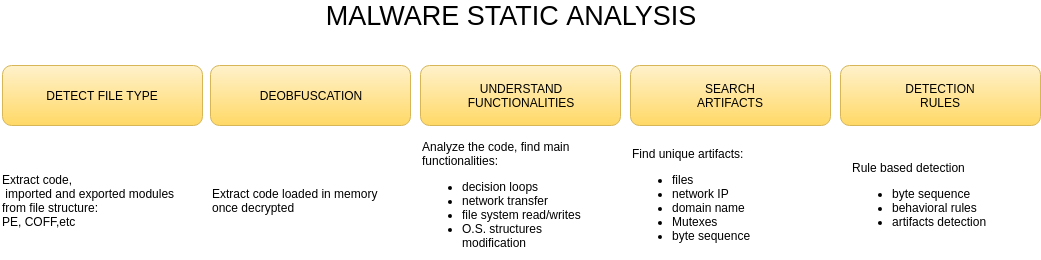
\includegraphics[scale=0.32]{./img/malware_static_analysis.png}
\end{figure}


Malware = malicious software, computer virus


% explain: reverse engineering malware (static analysis) = 
%             search for clues that help antivirus programs detect malicious code
%             like network communications, destination ip addresses,
%              destination domain names
%              files that are modified on the file system
%              mutexes (to avoid reinfection or multiple execution of the malicious code)
%             THE PROBLEM: It takes a lot of time
%             ONE


% Static because it involves reading code and not executing it and registering the events (which is another type of analysis)

% the task in the experiment 2 will try to help professionals working in stesp 3 and 4, which involv reading assembler code

\end{frame}





%------------------------------------------------------------------------
\begin{frame}{Experiment 2 - Compiled code function classification}{Context}

MALWARE STATIC ANALYSIS: understanding functionalities and searching for artifacts by analyzing assembler code.

% image of disassembled code:
%            ida pro free
%            a call to an unknown function 
%            code with comments on that call for example
%            function names and

\begin{figure}
    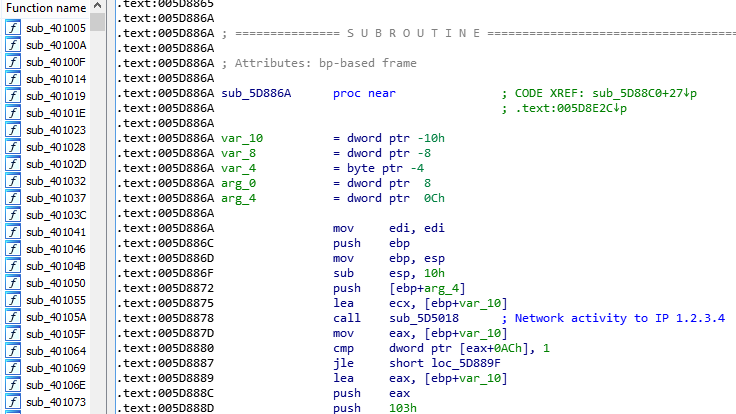
\includegraphics[scale=0.35]{./img/slides_exp2-context01c.png}
\end{figure}



% explain: compiled binary, 
%                - code that is transformed to an architecture dependent machine code
%                - so the processor can load it into memory and execute instruction by instruction
% explain: assembler language, 
%                % - allows to translated machine code directly into assembler language instructions
% explain: disassembler program,
%                - a program that reads a compiled code, interpres file structure and machine code into assembler language


\end{frame}




%------------------------------------------------------------------------
\begin{frame}{Experiment 2 - Compiled code function classification}{Context}


% explanation of the idea: rename function to help the analyst look faster for clues
Is it possible to rename the functions to help the analyst in searching specific functionalities within the code?


\begin{itemize}
    \item code2vec: Learning distributed representations of code (\citep{code2vec} )
    \item Learning to represent programs with graphs (\citep{139} )
\end{itemize}

% \nocite{code2vec} \nocite{139} 

% %\nocite{code2vec,129}
% \bibliographystyle{unsrt}
% \bibliography{references}


%code2vec uses abstract syntax trees to generate embeddings of functions that allow for later classification and then renaming of functions. It is performed on more complex syntax programming languages, with examples from free available code on github.

%Lergning to represent programs with graphs, they use GGNN to generate embeddings from snippets of code (again code availabe from github) and then they apply it for tasks like variable renaming.

% that was my source of inspiration: task inspiration form code2vec, gnn application comes from Allamanis paper.


\end{frame}




%------------------------------------------------------------------------
\begin{frame}{Experiment 2 - Compiled code function classification}{Goals and Motivation}

\begin{block}{Goal}{
       
        % Goal classify snipets of assembler code (subroutines or functions)
        Classify snippets of assembler code (subroutines or functions) into well known general purpose functionalities (Network, Disk, Encryption,etc)

    }\end{block}
    \begin{block}{Motivation}{
        Speed up the process of reverse engineering malicious code by adding some indications on the main functionality of assembler functions.
    }\end{block}
\end{frame}


%------------------------------------------------------------------------
\begin{frame}{Experiment 2 - Compiled code function classification}{Description}

% data gathering

% data transformation

\begin{figure}
    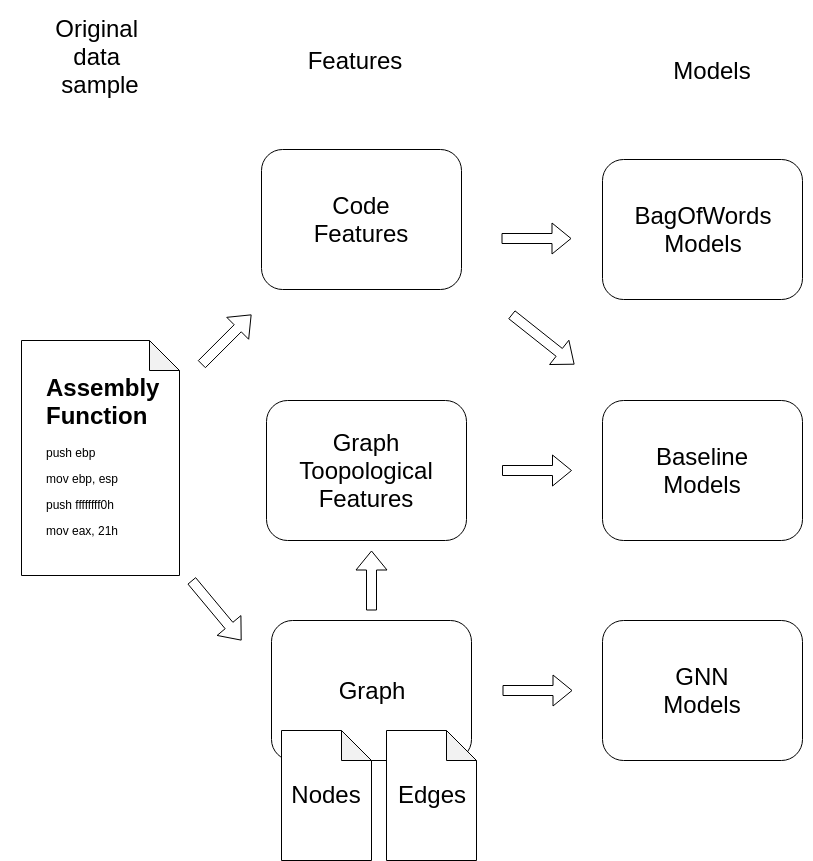
\includegraphics[scale=0.24]{./img/Features_and_models_diagram.png}
\end{figure} 


% There 3 main steps in this experiment, which are 
%  chosing a set software binaries and extracting their assembler language code
% finding a suitable labeling strategy

% then transforming this assembler language code into features for the algorithms: code features(counts of instructions, registers,), the graph of the code (a graph derrived from the execution flow of instructions and the operands of each instruction), and summary statistics of each graph (average node degree, or centrality measures).

% finally the models. The bagOfWOrds models are seentialy like the baseline but with a layer that will select the best parameters of the bag of words embedding
% hyper-parameter search using cross- validation (training and test splits and then k-fodl cross-validation)
% from more simple to more complex models
% goal is to see if gnn models can outperform more basic models




\end{frame}


%-----------------------------------------------------------------------
\begin{frame}{Experiment 2 - Compiled code function classification}{Description}

Generating and labeling the dataset



\begin{figure}[H]
\minipage{0.5\textwidth}

Code source:
\begin{itemize}
    \item Apache http server,
    \item Nginx http server,
    \item Filezilla fpt client,
    \item OpenSSL libraries,
    \item GlibC
\end{itemize}
\endminipage
\hfill
\minipage{0.5\textwidth}%
Compiled with debugging information (function names).\\

Original function names where grouped into class labels by a semi-automated rule-based keyword appearance procedure.
\\

Versions: v1 (10 classes), v2(120 classes), v3(24 classes)

\endminipage
\end{figure}



% assembler code file + debuggin info(function name)
% rule based label from 

% compilation with debugging information
%selected software: well-known Apache http, fielzill ftp client, nginx, httppser server, openssl and glibc


%number of classes in each approach

\end{frame}





%------------------------------------------------------------------------
\begin{frame}{Experiment 2 - Compiled code function classification}{Description}

% data gathering

% data transformation
Feature extraction


\begin{figure}[H]
\minipage{0.5\textwidth}%
  \centering
    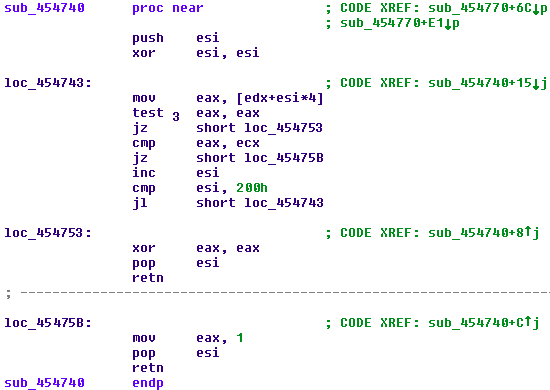
\includegraphics[width=0.9\linewidth]{img/code_graph02.png}
\endminipage
\minipage{0.5\textwidth}%
  \centering
    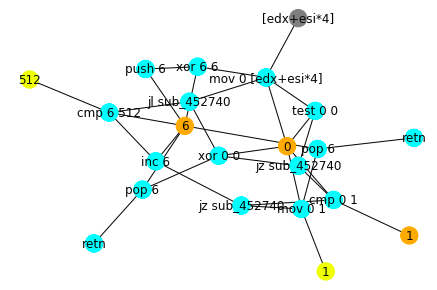
\includegraphics[width=0.9\linewidth]{img/code_graph01.png}
\endminipage
%\caption{Graph created from a fragment of assembler language code}
\end{figure}

\begin{itemize}
\item Extraction of features from code listing\\
\item Graph generation from the code listing\\
\item Extraction of topological features from the graph
\item Bag-of-words embedding (tokenization plus filtering by TF-IDF)
\end{itemize}
% graph of instructions created from the execution flow. 
% each instruction is linked to its previous and following instruction
% when jumps or calls are found, there is a link to a third instruction 
% operands of each instruction are also linked to it


\end{frame}



%------------------------------------------------------------------------
\begin{frame}{Experiment 2 - Compiled code function classification}{Description}

Machine learning models
%  Models used: describe quickly
\begin{itemize}
    % Baseline models
    \item \textbf{Baseline models}: Logistic Regression, Decision Trees, Random Forest, XGBoost, Neural Network (MLP). Code and graph topological features as input.

    % Bag of word with tf-idf
    \item \textbf{Bag-of-words models}: baseline models with Bag-of-word embedding filtered by TF-IDF as input

    % GNN: GCN, GraphSage, GIN, GGNN
    \item \textbf{Graph Neural Networks}: GCN, GraphSage, Gated Graph Neural Network, Graph Isomorphism Network. Graph as input.
\end{itemize}

\end{frame}


%------------------------------------------------------------------------
\begin{frame}{Experiment 2 - Compiled code function classification}{Results}

\begin{table}[H]

\adjustbox{max height=\dimexpr\textheight-5.9cm\relax,
           max width=0.99\textwidth, center}{

\centering
{\footnotesize
 \begin{tabular}{|llcccc|}
\hline
                   Model &               Features &  CV F1-macro &  Precision macro average &  Recall macro average &  F1-macro \\
\hline

MLP2 &   Code Bow and topological &     0.572 &                    0.350 &                 0.291 &     \textbf{0.299} \\

MLP4 &   Code Bow and topological &     0.528 &                    0.252 &                 0.251 &     0.237 \\

MLP2 &    Topological and code attr. &     0.420 &                    0.232 &                 0.203 &     0.186 \\

XGBoost &   Code Bow and topological &     0.387 &                    0.470 &                 0.374 &     \textbf{0.401} \\
                    
Random Forest &   Code Bow and topological &     0.307 &                    0.297 &                 0.293 &     \textbf{0.290} \\

Random Forest &    Topological and code attr. &     0.186 &                    0.246 &                 0.198 &     0.186 \\



XGBoost &           Topological &     0.171 &                    0.203 &                 0.190 &     0.190 \\



Random Forest  &           Topological&     0.164 &                    0.199 &                 0.187 &     0.186 \\


GIN &                  Graph &     0.147 &                    0.122 &                 0.180 &     0.145 \\



GGNN1 &                  Graph &     0.134 &                    0.052 &                 0.098 &     0.065 \\



\hline
\end{tabular}
}
}\label{FN_exp_v3}\caption{Function classification experiment results with dataset v1}
\end{table}



\end{frame}


%------------------------------------------------------------------------
\begin{frame}{Experiment 2 - Compiled code function classification}{Results}

\begin{table}[H]
\adjustbox{max height=\dimexpr\textheight-5.9cm\relax,
           max width=0.99\textwidth, center}{

\centering
{\footnotesize
 \begin{tabular}{|llrrrr|}
\hline
  Model &               Features &  CV F1-macro &  Precision macro average &  Recall macro average &  F1-macro \\
\hline
  MLP2 &   Code Bow and topological &     0.395 &                    0.224 &                 0.222 &     \textbf{0.213} \\
  MLP4 &   Code Bow and topological &     0.326 &                    0.141 &                 0.187 &     0.156 \\
  MLP3 &   Code Bow and topological &     0.313 &                    0.184 &                 0.176 &     0.151 \\
  
  %MLP2 &    Topological and code attr. &     0.228 &                    0.149 &                 0.147 &     0.129 \\
  
  RandomForest &   Code Bow and topological &     0.208 &                    0.288 &                 0.219 &     \textbf{0.209} \\
  
  XGBoost &    Topological and code attr. &     0.205 &                    0.236 &                 0.218 &     \textbf{0.221} \\
  
  %MLP2 &    Topological and code attr. &     0.197 &                    0.106 &                 0.125 &     0.095 \\
  
  GIN &           Graph &     0.199 &                    0.192 &                 0.205 &     0.198 \\

  %XGBoost &    Topological and code attr. &     0.192 &                    0.252 &                 0.214 &     \textbf{0.215} \\
  
  Random Forest &    Topological and code attr. &     0.179 &                    0.196 &                 0.181 &     0.178 \\
  
  Logistic Regression &   Code Bow and topological  &     0.173 &                    0.223 &                 0.202 &     0.188 \\
  %Random Forest &    Topological and code attr. &     0.168 &                    0.180 &                 0.179 &     0.175 \\
  

  

  XGBoost &           Topological &     0.108 &                    0.112 &                 0.116 &     0.112 \\
  
  RandomForest &           Topological &     0.102 &                    0.097 &                 0.104 &     0.098 \\
  GGNN1 &                  Graph &     0.064 &                    0.106 &                 0.103 &     0.080 \\
  
  %Logistic Regression &    Topological and code attr. &     0.059 &                    0.091 &                 0.088 &     0.064 \\
  
  %GGNN5 &                  Graph &     0.050 &                    0.030 &                 0.085 &     0.037 \\
                 
\hline
\end{tabular}
}
}\label{FN_exp_v3}\caption{Function classification experiment results with dataset v3}
\end{table}

\end{frame}

%------------------------------------------------------------------------
\begin{frame}{Experiment 2 - Compiled code function classification}{Conclusion}



\textbf{What are the key take aways?}
% conclusion on why topological features don't give as much signal as code features
% features vs classes boxplots?
\begin{itemize}
    \item Graph Neural Networks can be used for classification of code snippets
    \item Bag-of-word embedding carries more signal than the graph
    \item GNN training is highly influenced by how data is partitioned
    \item GNN training is costly
\end{itemize}

\end{frame}

%------------------------------------------------------------------------
\begin{frame}{Experiment 2 - Compiled code function classification}{Next steps}

\textbf{How can the results be improved?}
% improvements
\begin{itemize}
    \item Combine graphs with Bag-of-words embedding (node or graph level?)
    \begin{figure}[H]

      \centering
        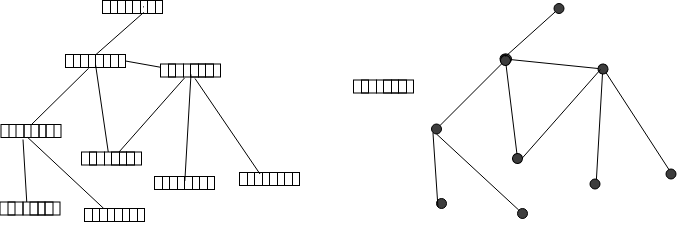
\includegraphics[width=0.9\linewidth]{img/exp2_improvements.png}

    \end{figure}

    \item Define a more constrained scenario, a more granular approach
\end{itemize}

\end{frame}


%------------------------------------------------------------------------
\section{Conclusion}
\begin{frame}{ }
\huge{4. Conclusion}
\end{frame}


%------------------------------------------------------------------------


\begin{frame}{Conclusion}%{Results summary}

\begin{itemize}
    \item Exploration of some Graph Neural Network models was successfully performed.
    \item Graph Neural Networks successfully applied to 2 problems. % even thought it has been methodologicaly proven that they were probably not the best models to use in both cases, plus experiment 2 problem was ill-posed or too ambitious and training resources were not enought for some kind
    \item The complexity of Graph Neural Network training has been observed.
    \item The need for a more thorough testing in experiment 1 has been stated.
    \item The need for a more constrained problem definition in experiment 2 has been stressed out.

\end{itemize}

\end{frame}



\begin{frame}[allowframebreaks]{References}

\bibliographystyle{unsrt}
\bibliography{references}


\end{frame}

\end{document}



% %------------------------------------------------------------------------
% \begin{frame}{Conclusion}{Next steps summary}

% \end{frame}



% %\nocite{*}












% %-----------------------------------------------------------------------------------------------------------------------------------------------------------------------------------------------------------------------------

% \section{Multivariate Analysis}

% %------------------------------------------------------------------------------
% \begin{frame}{Multivariate Analysis}{Dataset}
% Our initial dataset: House sales in king county
% \begin{table}[H]
\centering
\resizebox{\textwidth}{!}{
\begin{tabular}{lll}
\hline
\rowcolor[HTML]{C0C0C0} 
id             & a notation for a house                                                                                                                                 & Numeric \\
date           & Date house was sold                                                                                                                                    & String  \\
\rowcolor[HTML]{C0C0C0} 
price          & Price is prediction target                                                                                                                             & Numeric \\
bedrooms       & Number of Bedrooms/House                                                                                                                               & Numeric \\
\rowcolor[HTML]{C0C0C0} 
bathrooms      & Number of bathrooms/bedrooms                                                                                                                           & Numeric \\
sqft\_living   & square footage of the home                                                                                                                             & Numeric \\
\rowcolor[HTML]{C0C0C0} 
sqft\_lot      & square footage of the lot                                                                                                                              & Numeric \\
floors         & Total floors (levels) in house                                                                                                                         & Numeric \\
\rowcolor[HTML]{C0C0C0} 
waterfront     & House which has a view to a waterfront                                                                                                                 & Numeric \\
view           & Has been viewed                                                                                                                                        & Numeric \\
\rowcolor[HTML]{C0C0C0} 
condition      & How good the condition is ( Overall )                                                                                                                  & Numeric \\
grade          & \begin{tabular}[c]{@{}l@{}}overall grade given to the housing unit, \\ based on King County grading system\end{tabular}                                & Numeric \\
\rowcolor[HTML]{C0C0C0} 
sqft\_above    & square footage of house apart from basement                                                                                                            & Numeric \\
sqft\_basement & square footage of the basement                                                                                                                         & Numeric \\
\rowcolor[HTML]{C0C0C0} 
yr\_built      & Built Year                                                                                                                                             & Numeric \\
yr\_renovated  & Year when house was renovated                                                                                                                          & Numeric \\
\rowcolor[HTML]{C0C0C0} 
zipcode        & zip                                                                                                                                                    & Numeric \\
lat            & Latitude coordinate                                                                                                                                    & Numeric \\
\rowcolor[HTML]{C0C0C0} 
long           & Longitude coordinate                                                                                                                                   & Numeric \\
sqft\_living15 & \begin{tabular}[c]{@{}l@{}}Living room area in 2015(implies-- some renovations) \\ This might or might not have affected the lotsize area\end{tabular} & Numeric \\
\rowcolor[HTML]{C0C0C0} 
sqft\_lot15    & lotSize area in 2015(implies-- some renovations)                                                                                                       & Numeric \\ \hline
\end{tabular}%
}
\caption{Dataset's features - House sales in king county}
\label{table:dataFeatures}
\end{table}
% \end{frame}


% %------------------------------------------------------------------------------
% \begin{frame}{Multivariate Analysis}{Preprocessing}
% \begin{itemize}
%     \item \textbf{Missing data and Errors - } The dataset is complete (no blanks\textbackslash Na's) 
%     \item \textbf{Outliers - } Using Robustified Mahalanobis distance, we remove 8 individuals 
% \end{itemize}

% \begin{figure}
% 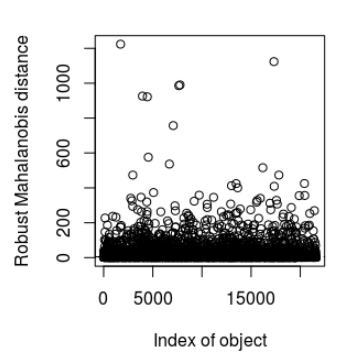
\includegraphics[scale=0.45]{./img/mahalanobis.png}
% \end{figure}

% \end{frame}


% %------------------------------------------------------------------------------
% \begin{frame}{Multivariate Analysis}{EDA: plots}

% \begin{figure}
% 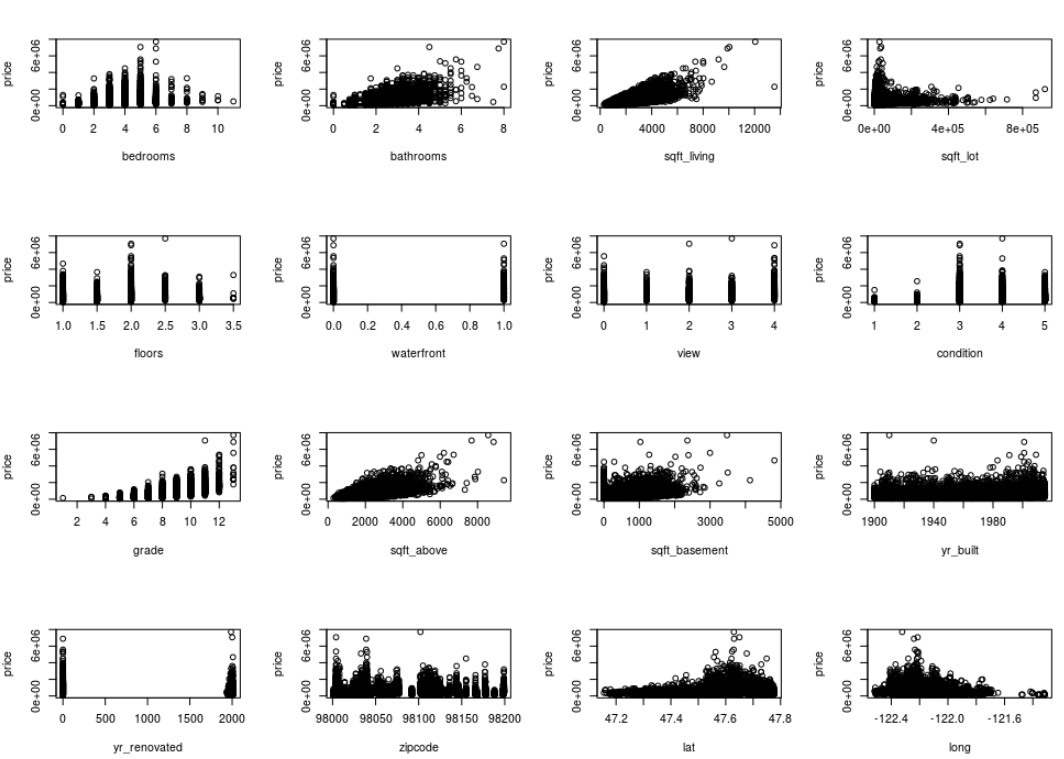
\includegraphics[scale=0.27]{./img/pairs-first.png}
% \end{figure}

% %We plot different variables of the dataset compared to the price, to start to graps what are the most important variables, what variables are possible candidates to be transformed.

% \end{frame}

% \begin{frame}{Multivariate Analysis}{EDA: histograms}

% \begin{figure}
% \includegraphics[scale=0.4]{./img/histograms.png}
% \end{figure}


% % we also plot histograms of each variables to see if they are drawn from a single distribution or not. etcetera
% \end{frame}


% %------------------------------------------------------------------------------
% \begin{frame}{Multivariate Analysis}{EDA: transformations}
% Logarithms and ratios
% \begin{figure}
% \includegraphics[scale=0.37]{./img/transformations.png}
% \end{figure}

% % here we have...
% %ratios capture same information in a lower dimension?
% %logs change the structure, correct skewness


% \end{frame}


% %------------------------------------------------------------------------------
% \begin{frame}{Multivariate Analysis}{EDA: transformations}
% Reducing skewness with logarithms.
% \begin{figure}
% \includegraphics[scale=0.32]{./img/log_skewness.png}
% \end{figure}

% %Logarithmic transformation can be useful to reduce skewness(for making patterns in the data more interpretable and for helping to meet the assumptions of inferential statistics). 
% % Not always worked so well.
% %>We also tried the Box-Cox transform, but didn't get better results than with this
% % we decided to create transformations for all continuous vars and then perform feature selection by experiments

% \end{frame}



% %------------------------------------------------------------------------------
% \begin{frame}{Multivariate Analysis}{EDA: correlation}
% For each highly correlated pair we remove one of the variables.
% \vspace*{-5pt}
% \begin{figure}
% 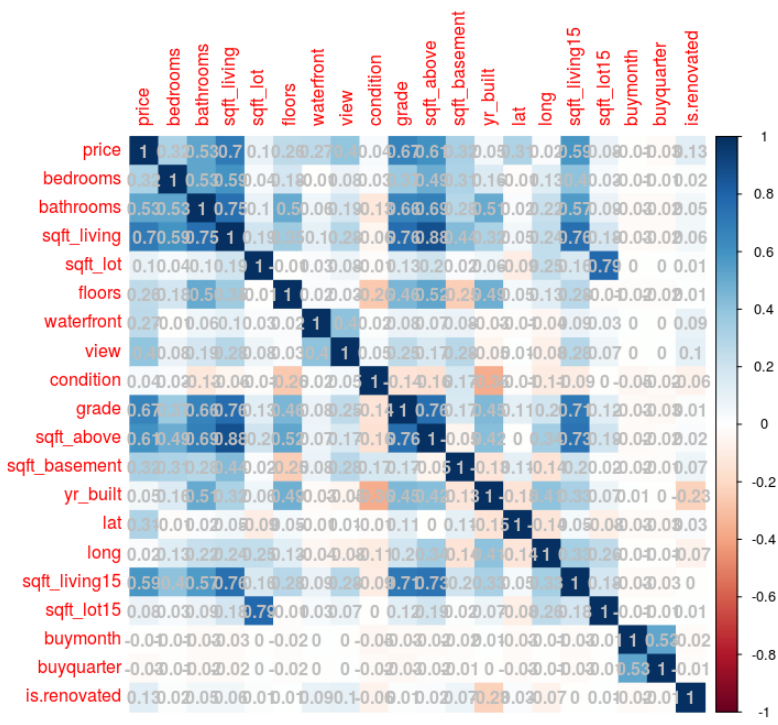
\includegraphics[scale=0.27]{./img/corr01.png}
% \end{figure}
% %\vspace*{-35pt}
% %we transform the variables using logarithms and ratios. sqft_living log transformation, bedroom/floor, floor/bathrooms, bathrooms/bedrooms = which can give an idea of the amount of money spent on the house, logarithm transform som echange of aspect.

% \end{frame}


% %------------------------------------------------------------------------------
% \begin{frame}{Multivariate Analysis}{EDA: correlation}
% For each highly correlated pair we remove one of the variables.
% \vspace*{-5pt}
% \begin{figure}
% \includegraphics[scale=0.27]{./img/corr02.png}
% \end{figure}
% %\vspace*{-35pt}
% % sqft_lot15/sqft_lot15, sqft_living15/sqft_living, sqft_above/sqft_living
% \end{frame}


% %------------------------------------------------------------------------------
% \begin{frame}{Multivariate Analysis}{EDA: correlation}
% For each highly correlated pair we remove one of the variables.
% \vspace*{-5pt}
% \begin{figure}
% \includegraphics[scale=0.25]{./img/corr03.png}
% \end{figure}
% %\vspace*{-35pt}

% \end{frame}



% %------------------------------------------------------------------------------
% \begin{frame}{Multivariate Analysis}{Unsupervised analysis: PCA}
% Correlations between variables and target(Price)
% \vspace*{-8pt}
% \begin{figure}
% 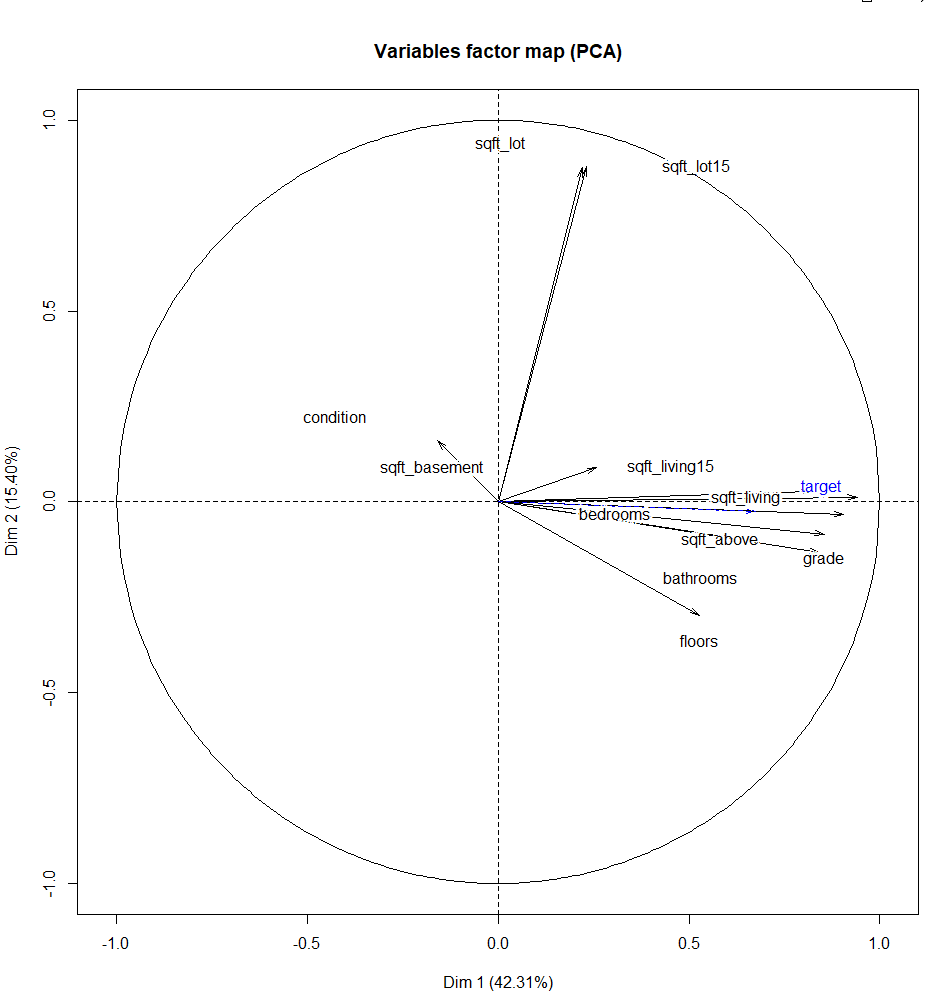
\includegraphics[scale=0.34]{./img/PCA.png}
% \end{figure}
% %sqft_lot not correlated (almost orthogonal)
% %the rest of continuous variables (sqft_living, bedrroms, sqft_above, grade, bathrroms) highly correlated between them and with the price
% % correlation between predictor variables is generally bad for training the models

% \end{frame}



% %------------------------------------------------------------------------------
% \begin{frame}{Multivariate Analysis}{Unsupervised analysis: Hierarchical Clustering}

% Assumption: only one cluster
% \begin{figure}
% 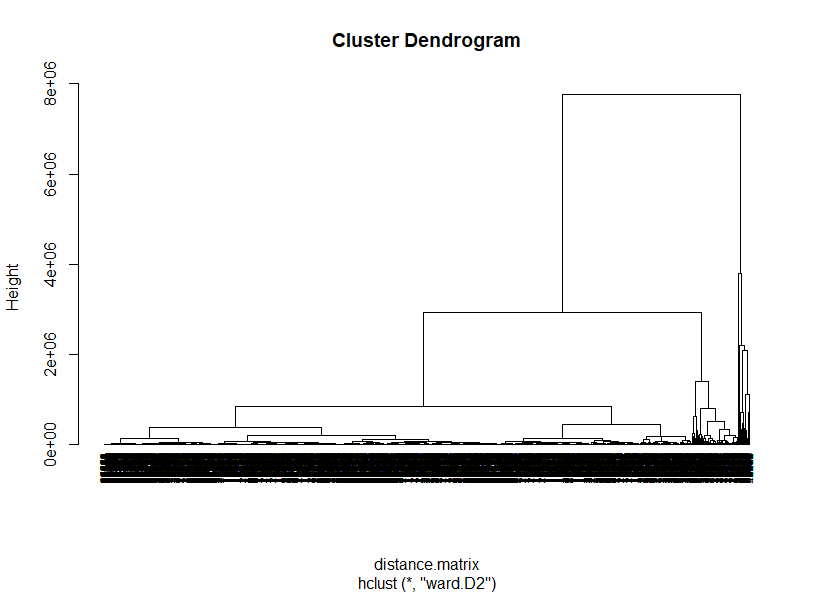
\includegraphics[scale=0.4]{./img/Hclustering.png}
% \end{figure}
% % worried about if there are different clusters for the data
% % after performing a hierarchycal clustering we conclude we can assume only one cluster
% % other wise, we would be forced to train different models for each cluster, and separate train and testing data according to the proximity to the centroid of each of the clusters.

% \end{frame}

% %Feature extraction
% %Feature extraction - logs, ratios: which ones
% %Feature extraction - correlation : the subsets we select 
% %Feature extraction - PCA  -> how we build the features + target


% \section{Feature Extraction}
% %------------------------------------------------------------------------------
% \begin{frame}{Feature Extraction}
% For each transformation: 
% \begin{itemize}
%     \item logarithms
%     \item ratios
%     \item removing highly correlated variables
%     \item significant principal components from PCA
% \end{itemize}
% we create new datasets by binding the new variables with the original target variable.

% \end{frame}


% %------------------------------------------------------------------------------
% \begin{frame}{Feature Extraction}
% Derived datasets:
% \input{./tables/datasets.tex}

% \end{frame}


% %models
% %Models - methodology
% %Models - selected models (maybe in one single slide all of them!)
% %Models - selected models - linear
% %Models - selected models - Ridge regression
% %Models - selected models - Lasso regression
% %Models - selected models - Decision trees for regression
% %Models - selected models - Random Forest for regression
% \section{Models}
% %------------------------------------------------------------------------------
% \begin{frame}{Models}{Methodology}

% Common training model methodology:
% \begin{itemize}
%     \item \textbf{Split dataset:} randomly split the training and test dataset 
%     \item \textbf{Model selection:}model selection(hyperparameters) by cross validation over the training set
%     \item \textbf{Refit:} refit of the model over all the training set with selected hyper parameters
%     \item \textbf{Generalization:} prediction of the model over test set to compute the testing error
% \end{itemize}
% We use the NRMSE.

% \end{frame}


% %------------------------------------------------------------------------------
% \begin{frame}{Models}{Methodology}

% Selected types of models:
% \begin{itemize}
%     \item Linear regression
%     \item Ridge regression
%     \item Lasso regression
%     \item Decision trees
%     \item Random forest
% \end{itemize}

% \end{frame}

% %Experiments
% %Experiments - overview
% %Experiments - initial exploration
% %Experiments - Feature selection
% %Experiments - Refinement
% %Experiments - Results
% \section{Experiments}
% %------------------------------------------------------------------------------
% \begin{frame}{Experiments \& Results}{Methodology overview}
% Our approach consists on exploration with final refinement:
% \begin{enumerate}
%     \item \textbf{Space exploration - }train all models, each with all the generated datasets and select the best 3.
%     \item \textbf{Feature selection - }for each model and dataset,
%     \item \textbf{Refit - }refit the best 3 models after feature selection.
% \end{enumerate}

% \end{frame}

% %------------------------------------------------------------------------------
% \begin{frame}{Experiments \& Results}{Space exploration}
% \vspace*{-5pt}
% Fragment of the experiments during exploration
% \vspace*{2pt}
% \input{./tables/exp_models_vs_featuresets_presentation.tex}
% \end{frame}

% %------------------------------------------------------------------------------
% \begin{frame}{Experiments \& Results}{Space exploration}
% Sorted plot of the validation, training and testing error (NRMSE)
% \vspace*{-7pt}
% \begin{figure}
% 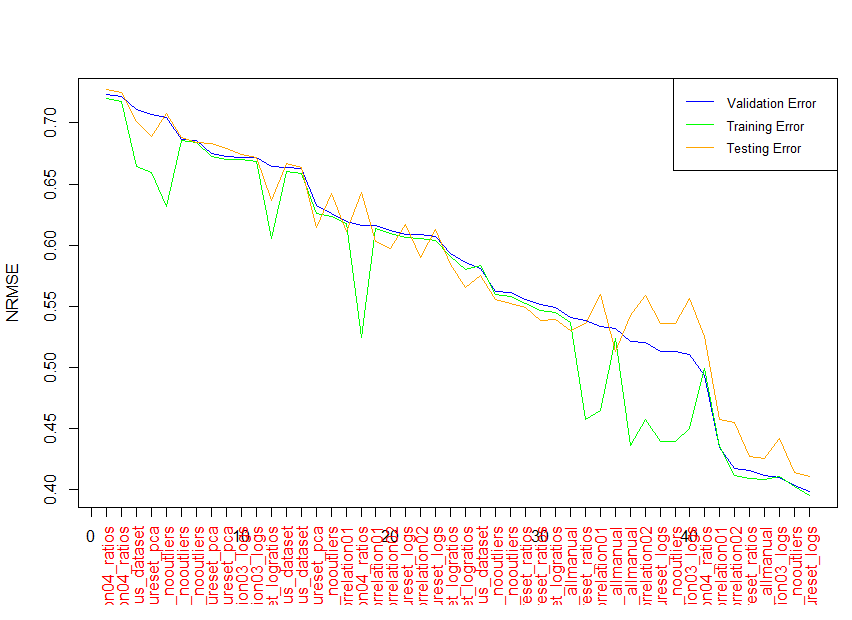
\includegraphics[scale=0.5]{./img/exp01.png}
% \end{figure}
% \end{frame}


% %------------------------------------------------------------------------------
% \begin{frame}{Experiments \& Results}{Space exploration}
% Selected models and datasets 
% \vspace*{3pt}
% % latex table generated in R 3.4.3 by xtable 1.8-2 package
% 
\begin{table}[H]
\begin{tabular}{cllcc}
  \hline
 & Model & Dataset & Validation NRMSE & Testing NRMSE \\ 
  \hline
  51 & regression\_randomforest & featureset\_logs & 0.40 & 0.41 \\ 
  42 & regression\_tree\_rpartlib & featureset\_nocorrelation03\_logs & 0.51 & 0.56 \\ 
  25 & lasso regression GLMNET & featureset\_allmanual & 0.53 & 0.51 \\ 
  
   \hline
\end{tabular}
\label{experiments}\caption{Experiments performed and their NRMSE for validation and testing }
\end{table}

% \end{frame}


% %------------------------------------------------------------------------------
% \begin{frame}{Experiments \& Results}{Feature selection}

% Evolution of the validation error in the Backward selection algorithm execution for the Lasso model. We had a minor improvement but in the end the dataset was smaller.
% \vspace*{-7pt}
% \begin{figure}
% \includegraphics[scale=0.3]{./img/lasso_SBS.png}
% \end{figure}

% \end{frame}


% %------------------------------------------------------------------------------
% \begin{frame}{Experiments \& Results}{Feature selection}

% Evolution of the validation error in the Backward selection algorithm execution for the Random Forest model.
% We can see that removing latitude or longitude has negative impact on the validation error whereas removing sqrt\_lot will reduce the validation error in 1\%.
% \vspace*{-7pt}
% \begin{figure}
% \includegraphics[scale=0.3]{./img/SBS.png}
% \end{figure}

% \end{frame}


% %------------------------------------------------------------------------------
% \begin{frame}{Experiments \& Results}{Refit \& Result}

% Final result
% \vspace*{3pt}
% \begin{table}[H]
\centering
\resizebox{\textwidth}{!}{
\begin{tabular}{cllccc}
  \hline
 & Model & Feature set & Validation.NRMSE & Training.NRMSE & Testing.NRMSE \\ 
  \hline
1 & regression\_tree\_rpartlib & featureset\_regression\_rpart\_tree\_fitting\_sfs & 0.51 & 0.45 & 0.56 \\ 
  2 & lasso regression GLMNET & featureset\_glmnet\_lasso\_sfs & 0.54 & 0.53 & 0.52 \\ 
  3 & regression\_randomforest & featureset\_regression\_randomforest\_sfs & 0.59 & 0.59 & 0.59 \\ 
   \hline
\end{tabular}
}
\caption{Best 3 models}
\label{table:final}
\end{table}
% \end{frame}



% %Conclusion
% %Conclusion - Presenting results
% %Conclusion - comparison of models/algorithms
% %Conclusion - Final impressions
% \section{Conclusion}
% %------------------------------------------------------------------------------
% %\begin{frame}{Conclusion}
% %    \begin{block}{\center Million dollar question}
% %    \center What is the best combination of feature set and model? 
% %    \end{block}
% %    \begin{block}{}
% %    Sequential forward selection performance:
% %    \begin{itemize}
% %        \item Choose sub-optimal feature set for random forest $\rightarrow$ that led to higher validation error.
% %        \item Decision trees and Lasso regression are less sensitive and SFS choose good feature set that preforms as good as found by exploration.
% %    \end{itemize}
% %    \end{block}
% %    \begin{block}{}
% %    During exploration RF overcome all other models. However, with SFS the generated forests under-preformed even compared to the decisions tree. 
% %    \end{block}
% %\end{frame}


% \begin{frame}{Conclusion}
%     \begin{block}{\center Million dollar question}
%     \center What is the best combination of feature set and model? 
%     \end{block}
%     \begin{block}{}
%     Sequential Backward selection performance:
%     \begin{itemize}
%         \item Random forest preformed better with smaller subset.
%         \item Decision trees and Lasso regression are less sensitive and SBS choose good feature set that preforms as good as found by exploration.
%     \end{itemize}
%     \end{block}
%     \begin{block}{}
%     During exploration RF overcome all other models and got even better performance using SBS.
%     Trying to use SFS, the generated RF under-preformed even compared to the decisions tree, it happens because the SFS lead to local minimum. 
%     \end{block}
% \end{frame}

% %------------------------------------------------------------------------------
% %\begin{frame}{Conclusion}
% %    \begin{block}{\center why?}
% %    What is the best combination of feature set and model? 
% %    \begin{itemize}
% %        \item  Random forest expected to be the best model $\rightarrow$ but highly dependent on the dataset.
% %        \item Decision trees and Lasso regression are less sensitive to the dataset.
% %    \end{itemize}
% %    \end{block}

% %\end{frame}

% %------------------------------------------------------------------------------
% \begin{frame}{Conclusion}{Future work}
% \begin{block}{Proposed improvements}
% \begin{itemize}
%     \item Test more advanced models: Splines, RVM, Bayesian approach to regression
%     \item Perform a deeper exploration of the possible features and combinations of features
%     \item Explore better feature selection methods: Bi-directional search, Plus-L Minus-R selection etc.
% \end{itemize}
% \end{block}
% \end{frame}

